\chapter{Wave equations on a graph}

In this chapter, we introduce the theoretical setup used to model light on a complex photonic network. This model is based largely on work done in \cite{Gaio2017}, which uses similar networks to study random lasing. We will start with the classial picture and introduce quantisation towards the end.

Since we are considering networks fabricated with single-mode waveguides, we treat light traveling through such networks as electromagnetic waves on a graph, i.e. waves conforming to the geometry of a specific network. 

Very simply, a graph is a collection of nodes i.e. points, $\{n_i\}$, and edges $\{E_{ij}\}$, lines that each connects two nodes together. These can be encoded in an adjacency matrix $A$, of dimension $N_n \times N_n$, $N_n$ being the number of nodes. $A_{ij} = A_{ji} = 1$ if there is an edge $E_{ij}$, and equals $0$ otherwise. For our purposes, we consider graphs that are directed ($E_{ij}$ and $E_{ji}$ are degenerate), planar (can be embedded onto a two-dimensional surface), and connected (every node has degree greater than zero).

The solutions are required to satisfy the wave equation
\begin{equation} \label{eq:wave_eq}
\frac{\partial^2 \Phi(x,t)}{\partial t^2} - v^2\frac{\partial^2 \Phi(x,t)}{\partial x^2} = 0
\end{equation}

where $v=c/n$ is the speed of light in the material. For silicon nitride waveguides, $n \approx 2$ \cite{Philipp1973}. Since the networks are linear, i.e. respond independently to different frequencies, we can look at Fourier components of the solution,
\begin{equation} \label{eq:k-space}
\Phi(x,w,t) \rightarrow \Psi(x,k)e^{-i\omega t}
\end{equation}
where $k=2\pi n/\lambda$ is the wavenumber. Assuming the dispersion relation $\omega = vk$, the $k$-components are required to satisfy the Helmholtz equation
\begin{equation} \label{eq:helmholtz_eq}
\frac{\partial^2 \Psi(x,k)}{\partial x^2} - k^2\Psi(x,k) = 0.
\end{equation}
The solutions (with time-dependence factored out) are therefore of the form of plane waves, 
\begin{equation}
\label{eq:planewave1}
\Psi(x,k) = X_+ e^{ikx} + X_- e^{-ikx}.
\end{equation}

For the purpose of waves on a graph, we use the coordinate $x \in [0, L_{ij}]$ on an edge $E_{ij}$ with length $L_{ij}$, and write the solution as
\begin{equation}
    \label{eq:planewave1edge}
    \Psi_{ij}(x,k) = X_{ij}e^{ikx} + X_{ji}e^{ik(L_{ij}-x)}.
\end{equation}

For a given $k$, the wave is therefore fully characterised by the two complex coefficients $X_{ij}$ and $X_{ji}$. Note that these solutions are oriented (we only consider $\Psi_{ij}$ and drop $\Psi_{ji}$, and the order of node indices are important) even though the edges are not. Furthermore, the wavenumber $k$ is allowed to be complex (with positive imaginary part) to capture absorption and loss along the waveguide.


\section{Continuity conditions}
The full solution for light on a network consists of a $\Psi_{ij}$ in the form of Eq.\ref{eq:planewave1edge} on each $E_{ij}$. The edges need to be consistently stitched together at the nodes. At each node, we impose the boundary conditions of a) continuity and b) zero divergence. More formally, at node $n_i$,
\begin{subequations}
\begin{align}
\label{eq:cont.cond}
        \Psi_{il} (x_i) &= \Psi_{im}(x_i) &&\forall l,m \rvert A_{il}=A_{im}=1\\
        \sum_m \frac{\partial\Psi_{im}(x)}{\partial x}\Big\rvert_{x_i} &= 0 &&\forall m \rvert A_{im}=1 
\end{align}
\end{subequations}

Where the derivative in condition b) is consistently in the outgoing direction. $x_i$ denotes the spatial location of $n_i$, and may be different for the coordinate used on each edge. Condition b) is equivalent to 
\begin{equation}
    \label{eq:in=out}
    \sum \Psi_{\textrm{ingoing}} (x_i) = \sum \Psi_{\textrm{outgoing}} (x_i).
\end{equation}

Enforcing these continuity conditions at each node amounts to a system of linear equations that fully constrain the $\{X_{ij},X_{ji}\}$ coefficients (cf. eq.\ref{eq:planewave1edge}). To see that this is true, suppose we have $N_e$ edges. Each node $n_i$, with corresponding degree $d_i$, contributes $d_i$ equations: $d_i - 1$ from pairwise continuity of the edges meeting at $n_i$ and $1$ from zero divergence. There are a total of $\sum_i{d_i} = 2N_e$ equations, since each edge connects two nodes and is counted twice.

A special case is the \textit{external} edges, i.e. those connected to nodes of degree one. The external (degree-one) nodes do not provide a sensible condition. However, this is amended by noticing that the coefficients going into the graph constitute the boundary condition, and can be specified by experimental parameters. For the purpose of this thesis, we set these in-going coefficients either equal to field injected into the networks, or equal to zero which correspond to the condition that external nodes do not reflect.

\section{Transmission matrix}
Given a network (graph), the experimentally accessible ports are the external edges. In contrast to conventional unidirectional photonic systems, each external edge is both an input and output port, and realistically it can serve as either. To model the \textit{transport} properties, we need to compute the input-output relations between these ports. These relations can be captured in a transmission matrix since the system is linear. Note however that the transmission matrix will be frequency-dependent since the continuity conditions will need to be solved independently for each $k$.

\subsection{Construction}
We construct the transmission matrix $T$ using the system of continuity equations in matrix form. First we arrange the $\{X_{ij},X_{ji}\}$ coefficients in a vector, such that the inputs (in-going coefficients on external edges) come first, followed by the outputs and the internal coefficients, denoted $X = (X_{in}, X_{out}, X_{other})^t$. The transmission matrix should be independent of the experimental input, so we drop the boundary conditions and only consider the equations arising from internal nodes. These can be written as a $(2N_e-N_{ext}) \times (2N_e)$ matrix $M$, $N_{ext}$ being the number of external edges, such that 
\begin{equation}
    \label{eq:Mopen}
    M\cdot X = 0.
\end{equation}

$M$ is of course in the same basis as that we picked for $X$, and can thus be written as 

\begin{equation}
\label{eq:M_AB}
M = \big{(}A \big{\rvert} B \big{)}
\end{equation}

Where $A$ is of size $(2N_e-N_{ext}) \times (N_{ext})$, and $B$ is $(2N_e-N_{ext}) \times (2N_e-N_{ext})$. Thus eq.\ref{eq:Mopen} becomes
\begin{subequations}
\begin{align}
    A\cdot X_{in} + B\cdot \begin{pmatrix}X_{out}\\X_{other}  \end{pmatrix}  &= 0 \\
    \begin{pmatrix}X_{out}\\X_{other}  \end{pmatrix} &= -B^{-1}A \cdot X_{in}
\end{align}
\end{subequations}

The transmission matrix between the input and output coefficients is therefore 
\begin{equation}
    \label{eq:T}
    T = (-B^{-1}A)_{1:N_{ext}},
\end{equation}
where the subscript on the right hand side signifies that we pick out only the rows corresponding to output ports.

\subsection{Responses and modes}
\label{sec:response_mode_def}
Notice that the matrix $-B^{-1}A$ from the previous section gives us information on all the coefficients as a function of the inputs. Although the internal edges are not experimentally accessible, they help us understand the behaviour of the network. We call $(X_{out},X_{other})^t$ the \textit{response} of $X_{in}$, and define the response matrix $R$:
\begin{equation}
    \label{eq:R}
    R = -B^{-1}A.
\end{equation}
We refer to the full vector $X=(X_{in},X_{out},X_{other})^t$ as the \textit{response mode} for a given $X_{in}$, or simply \textit{response} when the context is clear.

Transmission and response can be thought of as a dual picture to \textit{modes} of a network. To illustrate the concept, first consider a closed network with no inputs, i.e. with the boundary condition $X_{in}=0$. Then the matrix $M$ in Eq.\ref{eq:Mopen} is modified to have the form 
\begin{equation}
    \label{eq:Mclose}
    M = \begin{pmatrix}\mathbb{1} & \mathbb{0} \\
                        A         & B  \end{pmatrix}
\end{equation}
where $\mathbb{1}$ is the $N_{ext}\times N_{ext}$ identity matrix. Now $M$ is a square matrix. The modes of the closed network are the coefficients $X$ that solve Eq.\ref{eq:Mopen}, i.e., the null vector of $M$. Note that the null space of $M$ may be empty; and since $A$ and $B$ (and therefore $M$) are $k$-dependent, the modes of the closed network are discretised. The condition for having a non-trivial solution for $X$,
\begin{equation}
\label{eq:M_det}
    \textrm{det}[M(k)]=0,
\end{equation}
is satisfied only for a discrete set of $k$'s. We use the term ``mode'' to refer to both $k$'s that satisfy Eq.\ref{eq:M_det}, as well as their corresponding null vectors $X(k)$.

We go from a closed to an open network by allowing $X_{in}$ to be nonzero. In the mode (i.e. null vectors) picture, this means that some of the diagonal elements in the $\mathbb{1}$ on the top-left corner of Eq.\ref{eq:Mclose} are set to $0$, with indices corresponding to nonzero elements in $X_{in}$. In this case $M$ is no longer full rank and therefore has null vectors $X(k)$ for all $k$. However, if from one of the open edges we input a plane wave with $k$ resonant with a closed mode (Eq.\ref{eq:M_det} is satisfied), it is reasonable to expect the resulting response be similar to the closed mode $X(k)$, which already satisfies most of the continuity conditions for $k$ within the network. Indeed this is what we see using the model (Fig.\ref{fig:on_off_resonence_response}). On the other hand, the open input channels can be viewed as modifications to, or broadening of closed modes in the network. The modes capture inherent localisation properties of a given network geometry, which can be accessed by open channels to exhibit different transport properties. It is useful to keep this picture in mind, though for most of our discussions we will stick to the transmission and response picture, since inverting a smaller matrix is less computationally expensive than finding the determinants of a larger matrix. 
\begin{figure}[h]
  \centering
    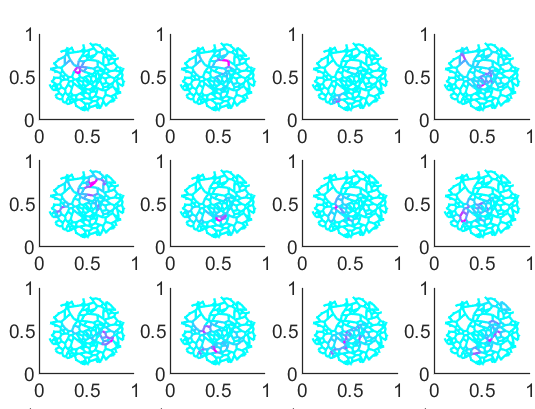
\includegraphics[width=0.6\textwidth]{ch2/fig2/randnet_passive_modes_examples.png}
    \caption{Example modes of a (closed) random network, computed by solving for Eq.\ref{eq:Mopen} and Eq.\ref{eq:M_det}. The average field intensity on each edge is displayed; warmer colour corresponds to higher intensity. We do not display the $k$ values since they are dependent on the scaling of network size. }
    \label{fig:closed_mode_examples}
\end{figure}
%\vspace{-2cm}
\begin{figure}[h]
    \centering
    \begin{subfigure}[b]{0.23\textwidth}
        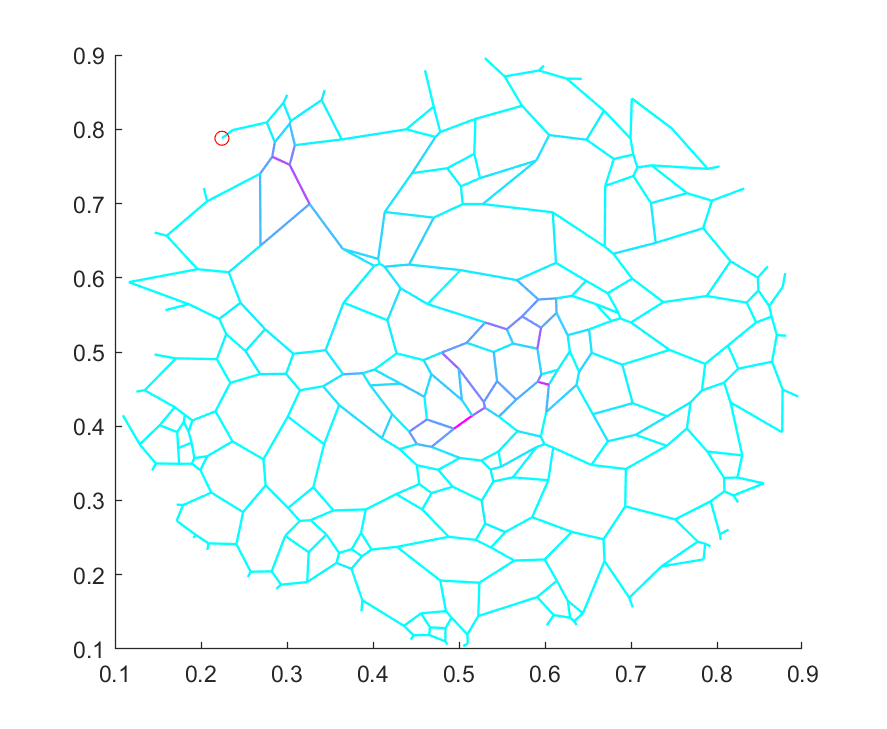
\includegraphics[width=\textwidth]{ch2/fig2/resonant_response_example.png}
        \caption{on-resonance}
        %\label{fig:gull}
    \end{subfigure}
~\quad\quad
    \begin{subfigure}[b]{0.23\textwidth}
        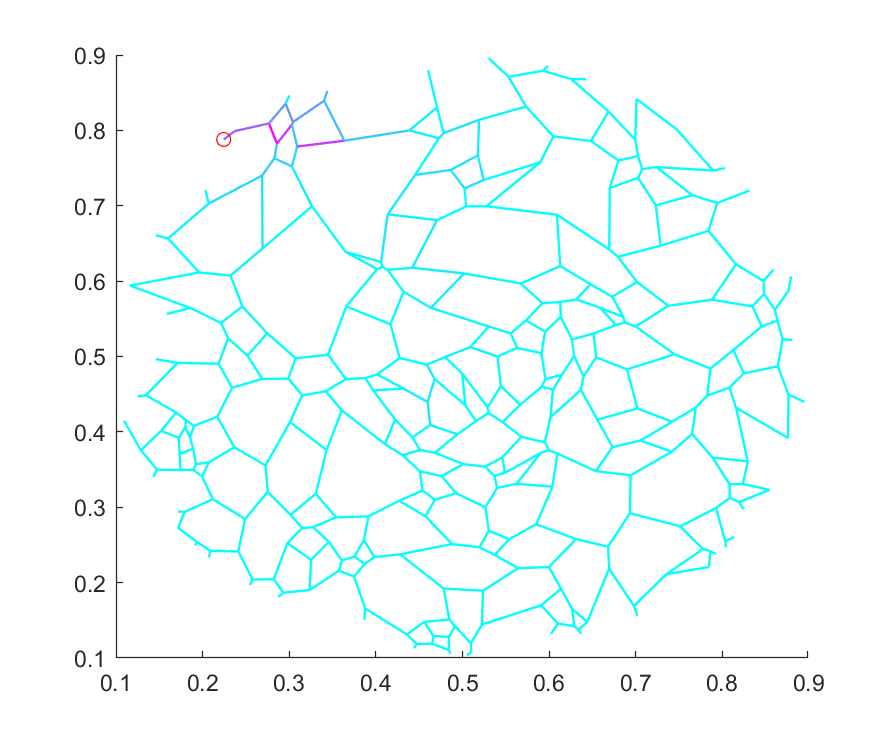
\includegraphics[width=\textwidth]{ch2/fig2/offresonant_response_example.png}
        \caption{off-resonance}
    \end{subfigure}
    
    \caption{Response modes of the network with a unit-intensity input at the edge labelled with a red circle. (a) input $k$ resonant with the closed mode corresponding to the top-right figure in Fig.\ref{fig:closed_mode_examples}. We see that (a) displays a response mode profile very similar to the closed mode, while in (b) the input is reflected without traversing much of the network.}\label{fig:on_off_resonence_response}
\end{figure}

%\vspace{5cm}
\pagebreak

\section{Physical picture}
\label{sec:physical_picture}
It is evident from our construction of the wave-on-a-graph model that this is a vastly simplified description of light on nanophotonic networks. For one, we have not taken into account the mode shape of light within the waveguides, and are ignoring any potential higher modes or frequency-dependent mode behaviours. We have also ignored any nonlinear dispersion relation between $\omega$ and $k$ in our representation of the plane wave components. However, it is a basic framework to help us simulate light transport through such networks, as a function of the spatial and spectral profile of the input.

The networks and graphs in question are large, complex systems, and it is helpful to think in analogy to simpler, more familiar physical systems. For example, we can think of each edge in a network as a one-dimensional Fabry-P\'erot cavity, which simply consists of a pair of leaky flat mirrors. Along each edge, or within each cavity, light can propogate in both directions, and can reflect or leak out at the nodes/mirrors. A network can thus be viewd as a collection of coupled Fabry-P\'erot cavities, where the way light leaked from one cavity is injected into another is specified by our continuity conditions. Alternatively, we can think of a network as a collection of ring resonators, where the plane waves of a certain $k$ must be configured in such a way that is compatible on the overlapping edges of adjacent rings.


\begin{figure}[h]
    \centering
    \begin{subfigure}[b]{0.3\textwidth}
        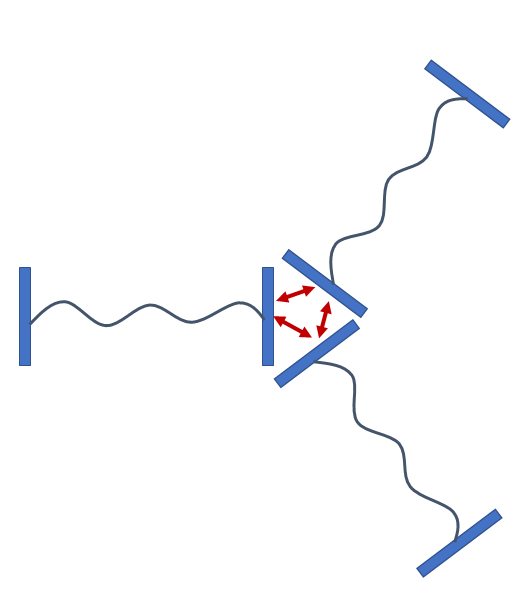
\includegraphics[width=\textwidth]{ch2/fig2/coupled_FP.png}
        \caption{}
        %\label{fig:gull}
    \end{subfigure}
~\quad\quad
    \begin{subfigure}[b]{0.3\textwidth}
        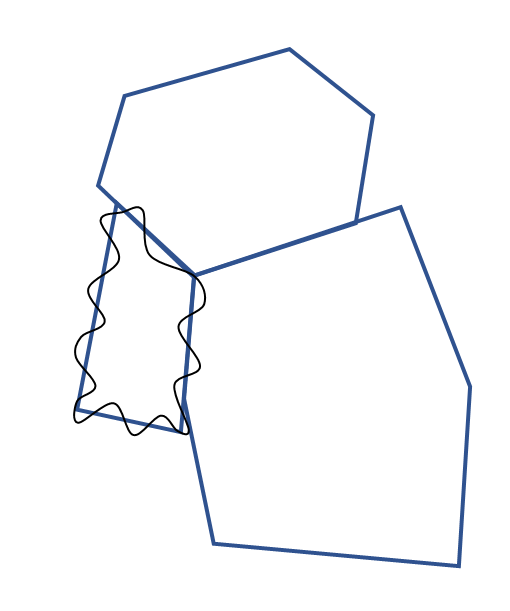
\includegraphics[width=\textwidth]{ch2/fig2/coupled_rings.png}
        \caption{}
    \end{subfigure}
    
    \caption{We can think of our wave-on-a-graph model as a) a collection of coupled 1D Fabry-P\'erot cavities or b) a collection of coupled ring resonators.}\label{fig:coupled_FP_rings}
\end{figure}

These analogies are helpful in interpreting the physical meaning of transport features in a network. In particular, although the $k$ modes obtained by solving Eq.\ref{eq:M_det} are discrete, in the coupled-cavities picture we can consider broadening of the modes, i.e. finite Q factors. For example, the $k$ modes with a larger imaginary part correspond to more lossy modes. In the response modes picture, the network modes are broadened by coupling to the input channels.


\section{Toy examples}
\label{sec:toy_examples}

In this section we will explicitly construct the $M$ and $T$ matrices of several toy examples. One advantage of such small systems is that we are able to write down the analytic expressions for $T$, thus showing the functional dependence of transmission on $k$. These examples will also help elucidate basic principles of how network structure affects transmission.

\begin{figure}[h]
  \centering
    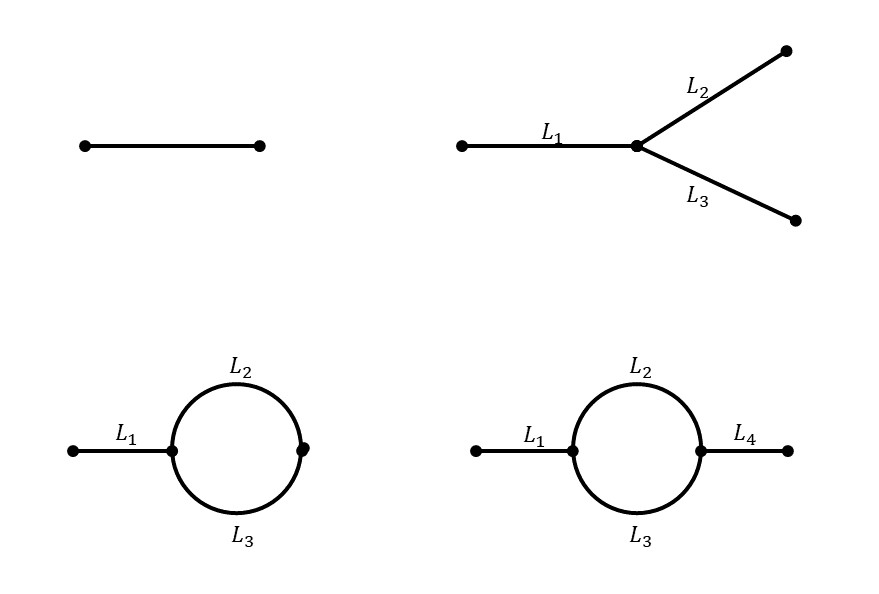
\includegraphics[width=0.65\textwidth]{ch2/fig2/toy_examples_labeled.jpg}
    \caption{Some toy example networks we consider: line, 3-prong, tadpole, and Saturn. The edges are labelled by their corresponding lengths.}
    \label{fig:toy_examples}
\end{figure}

The most trivial example is a graph of one edge connecting two nodes, i.e. a network that simply consists of one open waveguide. In this case there is nothing to solve since the only edge is open, and plane wave of any frequency is allowed to propagate in both directions.

Next we consider the 3-prong network, which consists of three open edges meeting at one internal node. Picking a basis where the first three indices are input coefficients and the last three are outputs, the continuity conditions can be represented as a matrix $M$ in the same form as Eq.\ref{eq:M_AB}, where

\begin{equation}
    \label{eq:AB_3prong}
    A = \begin{pmatrix}
    e^{ikL_1} & -e^{ikL_2} & 0           \\[0.3em]
       e^{ikL_1} & 0           & -e^{ikL_3} \\[0.3em]
       e^{ikL_1}  & e^{ikL_2} & e^{ikL_3} \end{pmatrix}, \quad
    B = \begin{pmatrix}
        1 & -1 & 0           \\[0.3em]
        1 & 0 & -1 \\[0.3em]
        -1  & -1 & -1 \end{pmatrix}
\end{equation}

from which we can compute the transmission
\begin{equation}
    \label{eq:T_3prong}
    T = \begin{pmatrix}
    -\frac{1}{3}e^{ikL_1} & \frac{2}{3}e^{ikL_2} & \frac{2}{3}e^{ikL_3} \\[0.3em]
    \frac{2}{3}e^{ikL_1} & -\frac{1}{3}e^{ikL_2} & \frac{2}{3}e^{ikL_3} \\[0.3em]
    \frac{2}{3}e^{ikL_1}  & \frac{2}{3}e^{ikL_2} & -\frac{1}{3}e^{ikL_3} \end{pmatrix}.
\end{equation}

The transmission matrix is symmetric for the three edges as expected. Given a unit-amplitude input on a certain edge, $1/3$ is reflected, while the other two edges each gets a $2/3$ amplitude output. This illustrates another caveat of our wave-on-a-graph model, that it does not take into account the angles at which edges meet at a node. Realistically, the transmission vs. reflection ratio would depend on the angle. Most of the light sent in through an edge would be reflected if the two other edges are perpendicular to it, while most would be transmitted if the two outputs are at a small angle from the input edge. However, equal power splitting at nodes have been observed in similar resonant waveguide networks with more regular geometries \cite{Feigenbaum2010}.

To introduce $k$-dependent behaviour into our networks, we need to include closed loops. The simplest example is the tadpole geometry, with one closed ring connected to one external edge. An extra node is introduced along the ring to avoid non-zero entries on the diagonal of the adjacency matrix. We can again write down  

\begin{equation}
    \label{eq:AB_tadpole}
    \hspace{-3cm}
    A = \begin{pmatrix}
        e^{ikL_1}  \\[0.3em]
        e^{ikL_1}  \\[0.3em]
        0          \\[0.3em]
        0          \\[0.3em]
        e^{ikL_1}   \end{pmatrix}, 
      % \hspace{-5cm}
      \quad
    B = \begin{pmatrix}
    1 & -1 & -e^{ikL_2} & 0 & 0 \\[0.3em]
    1 & 0 & 0 & -1 & -e^{ikL_3} \\[0.3em]
    0 & e^{ikL_2} & 1 & -e^{ikL_3} & -1 \\[0.3em]
    0 & e^{ikL_2} & -1 & e^{ikL_3} & -1 \\[0.3em]
    -1 & -1 & -e^{ikL_2} & -1 & e^{ikL_3} 
     \end{pmatrix},
     \hspace{-3cm}
\end{equation}
where the basis is such that the input coefficient is in the first coordinate, the output is in the second, and the third through sixth are internal. In this case the transmission is just a scalar
\begin{equation}
    \label{eq:T_tadpole}
    T=\frac{e^{ikL_1}-3e^{ikL}}{e^{ikL}-3},
\end{equation}
where $L=L_1+L_2+L_3$. It is easy to verify that $T$ has unit intensity, i.e. the output is a reflection of the input with a $k$-dependent phase.
\begin{figure}[h]
  \centering
    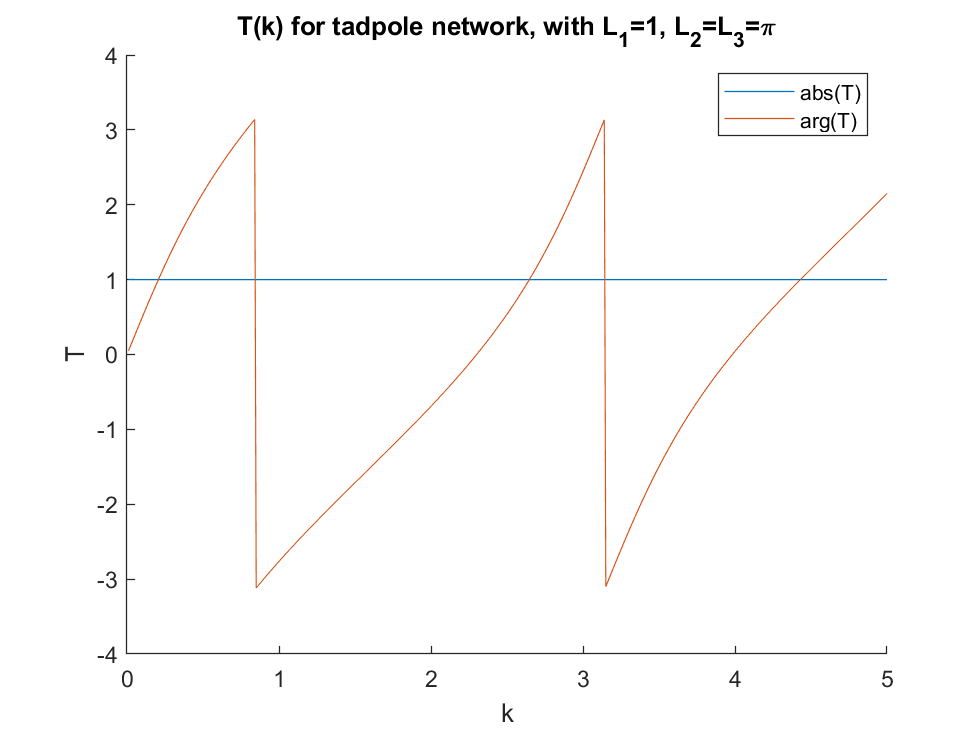
\includegraphics[width=0.6\textwidth]{ch2/fig2/tadpole_T.png}
    \caption{Transmission of the tadpole network with $L_1=1$, $L_2=L_3=\pi$. It is a phase factor that varies continuously with $k$, since the jumps from $\pi$ to $-\pi$ are an artefact of the branch cut.}
    \label{fig:T_tadpole}
\end{figure}

In an experiment, it is unrealistic to measure input and output at the same port. We therefore extend the tadpole example to Saturn by attaching another external edge to the loop. Technically we would want another node along the loop to avoid a double connection between the nodes, but it is easy to verify that enforcing continuity conditions at a degree-2 node is equivalent to having a single waveguide. We therefore keep the present geometry for simplicity. The $A$, $B$ matrices are similar to the tadpole network and will be omitted. Setting  $L_1=L_2=L_3=L_4=1$ to simplify the expression,
\begin{equation}
    \label{eq:T_saturn}
    T  = \begin{pmatrix}
        T_{LL} & T_{RL}\\[0.3em] 
        T_{LR} & T_{RR} 
          \end{pmatrix}
    = \begin{pmatrix}
        \frac{-3e^{ik}(e^{i2k}-1)}{e^{i2k}-9} & \frac{-8e^{i2k}}{e^{i2k}-9}\\[0.3em] \frac{-8e^{i2k}}{e^{i2k}-9} & \frac{-3e^{ik}(e^{i2k}-1)}{e^{i2k}-9}
          \end{pmatrix},
\end{equation}
where $T_{LR}$ is the component of input from the left that is transmitted to the right, etc. Again, we see the expected symmetry between the input ports, and $k$-dependent transport behaviour.

\begin{figure}[h]
  \centering
    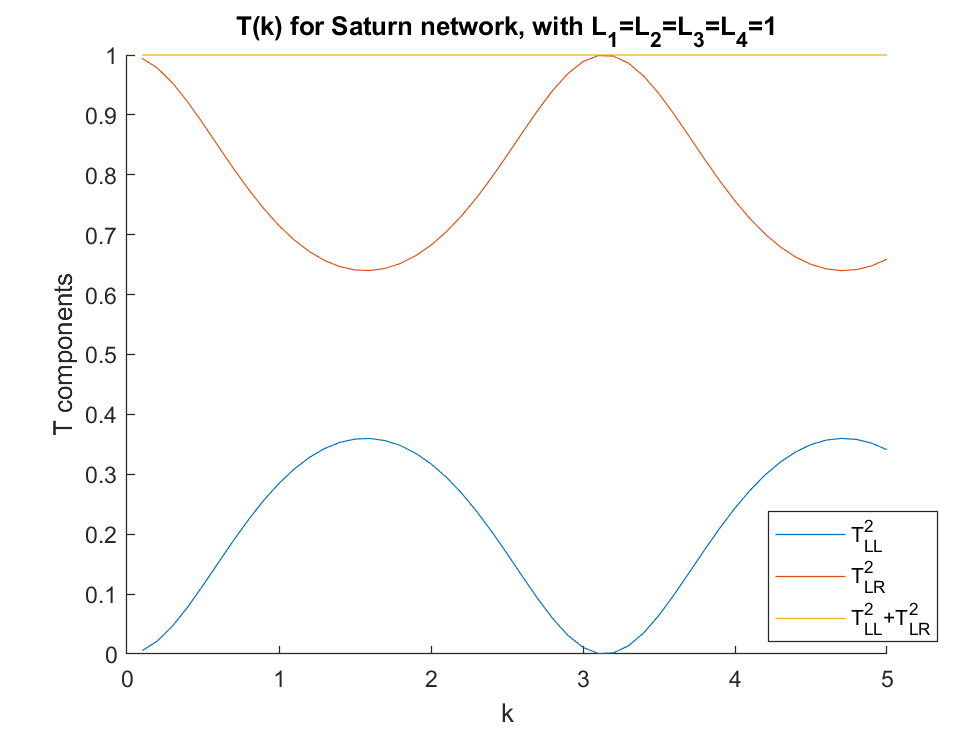
\includegraphics[width=0.6\textwidth]{ch2/fig2/saturn_T.png}
    \caption{Transmission and reflection intensities of the Saturn network with $L_1=L_2=L_3=L_4=1$. We see both graphically and analytically from Eq.\ref{eq:T_saturn} that we get unit transmission and zero reflection when $k$ is an integer multiple of $\pi$.}
    \label{fig:T_saturn}
\end{figure}

A full complex network is a connected collection of small components similar to the four considered here. From these toy examples we see that nodes divide incoming amplitudes into outgoing amplitudes in all directions, and that closed loops determine the frequencies which are transmitted or reflected in a region of the network. Interference on top of these simple effects gives rise to the rich transport properties of complex photonic networks.  


\section{Quantisation}
The theory established so far applies to the Fourier components of classical electromagnetic waves. Since we want to use complex photonic networks as a platform for LOQC and quantum light state engineering, it is necessary to introduce a quantised version of our model.

Analogously to linear optical components such as beam splitters, we want the scattering process (i.e. transmission matrix) to act the same way on classical and quantum light. For example, in the quantum optical description of a beam splitter, an input mode (and its corresponding bosonic creation operator) undergoes a unitary transformation, which turns it into a linear combination of the two output modes:
\begin{equation}
    \label{eq:beamsplitter}
    a_i^\dagger \rightarrow Ua_i^\dagger U^\dagger = S_{i1}a_1^\dagger + S_{i2}a_2^\dagger
\end{equation}
with $i=1,2$. The linear transformation matrix $S$ with components specified as above is unitary, and is the same scattering matrix that acts on classical inputs. By direct analogy, we would like to use the $T$ we have constructed for each network the same way as $S$. This approach is indeed the one we will employ, but it warrants some physical justification.

To interpret the meaning of this quantisation approach within the network, we return to the coupled cavity picture introduced in section \ref{sec:physical_picture}. Optical cavities, and Fabry-P\'erot cavities in particular, are commonly treated using the system-and-bath Hamiltonian of the form \cite{Zandi2012}
\begin{align}
\label{eq:H_fabryperot}
        H &= H_{cavity} + H_{field} + H_{interaction}\\ \nonumber
          &= \sum_n \hbar\omega_n(a_n^\dagger a_n) + \int dk [\hbar vk  (a^\dagger(k)a(k))] + \sum_n\int dk (\mu a^\dagger(k)a_n) + h.c.
\end{align}
where $\mu$ denotes the coupling strength, usually put in as an empirical factor. There are various theoretical methods to quantise optical cavities, including the input-output formalism, mode-of-the-universe descriptions, and Green's function approaches \cite{Barlow2015}. The Feshbach projector technique has been used to specifically investigate the field quantisation for light scattered by disordered dielectric media \cite{Viviescas2003}, and reproduced the same systems-and-bath Hamiltonian from rigorous analysis. 

The system-and-bath Hamiltonian is phenomenologically consistent with our  classical model: we have a discrete set of modes in the closed network (labeled by $\{\omega_n\}$ in Eq.\ref{eq:H_fabryperot}), and a continuous set of free fields that can couple to it. One caveat is that for an open network we can always solve $M\cdot X=0$ (Eq.\ref{eq:Mopen}), i.e., we can find a response mode in the network for any $k$. Although there is a qualitative difference between nonresonant response and resonant modes (Fig.\ref{fig:on_off_resonence_response}), they are treated on the same footing, and we do not have a quantitative model for how the mode widths are determined by coupling to open channels. The result in \cite{Viviescas2003} states that the systems-and-bath Hamiltonian is only reproduced for narrow modes, otherwise it will contain terms of the form $a_{cavity}a_{field}$ or $a_{cavity}^\dagger a_{field}^\dagger$. However, we expect randomness in the networks to produce highly frequency-dependent behaviour; numerical simulations in the following chapter indeed display narrow transmission peaks for low-loss systems. 

The quantised picture for light scattering through complex networks is thus as follows: a photon $a^\dagger(x,k)$ entering a network adds one excitation to the response mode for that input port $x$, characterised by $R(k)$. The response mode is in turn coupled to a collection of output channels, formally written as 
\begin{equation}
\label{eq:output_wf}
    T(x,k)=\sum_j c_j a_j^\dagger,
\end{equation}
where the output coefficients have been interpreted as output wavefunction amplitudes $c_j$, with $j$ ranging over the output ports. We have slightly abused notation here ($T$) since the $c_j$ values will simply correspond to columns in the classical transmission matrix. Note that although we have compared individual edges in the network to Fabry-P\'erot cavities, the mode excitations are for the network as a whole. This is because we want the quantum picture to be consistent with classical Maxwell's equations, where the field amplitude on each edge is fixed relative to each other by the continuity conditions. Therefore the fields on each edge cannot be quantised individually, since in the quantum regime the continuous field amplitudes of a plane wave become quantised (i.e. discrete) field excitations. 

As discussed above, one way network excitations are treated differently than optical cavities is that the responses and modes are treated on equal formal footing. This can be viewed as networks being ``cavities'' with ``soft boundaries'', where the reflected inputs still traverse a small section of the network. Similarly, localisation effects lead to difference in size even in the true modes of a network. Therefore our analogy with cavities is not perfect. However, a detailed description of the internal dynamics is not necessary since transport phenomena only concern external edges. We thus return to the original comparison with beam splitters, where a network is viewed as one optical element which performs $k$-dependent, linear mixing of spatial modes. In this zoomed-out picture, all the quantum effects come from either the quantum nature of input light, or interference between output wavefunctions. 

An alternative approach more similar to conventional LOQC systems introduces a scattering matrix at each node; the overall scattering matrix is the the tensor product of those at each node. Then the light mode on each network edge is exactly that on a waveguide, and the scattering behaviour at each node is of the same nature as beam splitters. This approach is similar to the random matrix model for multiple scattering \cite{Rotter2017}, and has been employed to model small networks of two or three nodes \cite{Lepri2017}. Instead of field continuity conditions at each node, the consistency of this network setup is enforced by a determinant condition on the scattering matrix, as well as a matrix describing wave propagation along the edges. This is the same condition used in the theory of abstract quantum graphs \cite{Gnutzmann2006}. A further advantage of the scattering matrix formalism is that it can account for asymmetric scattering effects at each node, which is ignored by our current model (cf. the 3-prong network example in section \ref{sec:toy_examples}). The main constraint preventing us from using this approach is computational expense: to explore the localisation effect in complex networks, we need systems of hundreds up to few thousand nodes. It is difficult to solve determinant equations for large systems, particularly since they will be $k$-dependent; there is furthermore the computational overhead to determine the scattering matrix at each node using, for example, finite-difference time-domain (FDTD) methods. Nevertheless the scattering matrix formalism is a valid model for photonic networks and remains a possible route for future investigation.
